\documentclass[1p]{elsarticle_modified}
%\bibliographystyle{elsarticle-num}

%\usepackage[colorlinks]{hyperref}
%\usepackage{abbrmath_seonhwa} %\Abb, \Ascr, \Acal ,\Abf, \Afrak
\usepackage{amsfonts}
\usepackage{amssymb}
\usepackage{amsmath}
\usepackage{amsthm}
\usepackage{scalefnt}
\usepackage{amsbsy}
\usepackage{kotex}
\usepackage{caption}
\usepackage{subfig}
\usepackage{color}
\usepackage{graphicx}
\usepackage{xcolor} %% white, black, red, green, blue, cyan, magenta, yellow
\usepackage{float}
\usepackage{setspace}
\usepackage{hyperref}

\usepackage{tikz}
\usetikzlibrary{arrows}

\usepackage{multirow}
\usepackage{array} % fixed length table
\usepackage{hhline}

%%%%%%%%%%%%%%%%%%%%%
\makeatletter
\renewcommand*\env@matrix[1][\arraystretch]{%
	\edef\arraystretch{#1}%
	\hskip -\arraycolsep
	\let\@ifnextchar\new@ifnextchar
	\array{*\c@MaxMatrixCols c}}
\makeatother %https://tex.stackexchange.com/questions/14071/how-can-i-increase-the-line-spacing-in-a-matrix
%%%%%%%%%%%%%%%

\usepackage[normalem]{ulem}

\newcommand{\msout}[1]{\ifmmode\text{\sout{\ensuremath{#1}}}\else\sout{#1}\fi}
%SOURCE: \msout is \stkout macro in https://tex.stackexchange.com/questions/20609/strikeout-in-math-mode

\newcommand{\cancel}[1]{
	\ifmmode
	{\color{red}\msout{#1}}
	\else
	{\color{red}\sout{#1}}
	\fi
}

\newcommand{\add}[1]{
	{\color{blue}\uwave{#1}}
}

\newcommand{\replace}[2]{
	\ifmmode
	{\color{red}\msout{#1}}{\color{blue}\uwave{#2}}
	\else
	{\color{red}\sout{#1}}{\color{blue}\uwave{#2}}
	\fi
}

\newcommand{\Sol}{\mathcal{S}} %segment
\newcommand{\D}{D} %diagram
\newcommand{\A}{\mathcal{A}} %arc


%%%%%%%%%%%%%%%%%%%%%%%%%%%%%5 test

\def\sl{\operatorname{\textup{SL}}(2,\Cbb)}
\def\psl{\operatorname{\textup{PSL}}(2,\Cbb)}
\def\quan{\mkern 1mu \triangleright \mkern 1mu}

\theoremstyle{definition}
\newtheorem{thm}{Theorem}[section]
\newtheorem{prop}[thm]{Proposition}
\newtheorem{lem}[thm]{Lemma}
\newtheorem{ques}[thm]{Question}
\newtheorem{cor}[thm]{Corollary}
\newtheorem{defn}[thm]{Definition}
\newtheorem{exam}[thm]{Example}
\newtheorem{rmk}[thm]{Remark}
\newtheorem{alg}[thm]{Algorithm}

\newcommand{\I}{\sqrt{-1}}
\begin{document}

%\begin{frontmatter}
%
%\title{Boundary parabolic representations of knots up to 8 crossings}
%
%%% Group authors per affiliation:
%\author{Yunhi Cho} 
%\address{Department of Mathematics, University of Seoul, Seoul, Korea}
%\ead{yhcho@uos.ac.kr}
%
%
%\author{Seonhwa Kim} %\fnref{s_kim}}
%\address{Center for Geometry and Physics, Institute for Basic Science, Pohang, 37673, Korea}
%\ead{ryeona17@ibs.re.kr}
%
%\author{Hyuk Kim}
%\address{Department of Mathematical Sciences, Seoul National University, Seoul 08826, Korea}
%\ead{hyukkim@snu.ac.kr}
%
%\author{Seokbeom Yoon}
%\address{Department of Mathematical Sciences, Seoul National University, Seoul, 08826,  Korea}
%\ead{sbyoon15@snu.ac.kr}
%
%\begin{abstract}
%We find all boundary parabolic representation of knots up to 8 crossings.
%
%\end{abstract}
%\begin{keyword}
%    \MSC[2010] 57M25 
%\end{keyword}
%
%\end{frontmatter}

%\linenumbers
%\tableofcontents
%
\newcommand\colored[1]{\textcolor{white}{\rule[-0.35ex]{0.8em}{1.4ex}}\kern-0.8em\color{red} #1}%
%\newcommand\colored[1]{\textcolor{white}{ #1}\kern-2.17ex	\textcolor{white}{ #1}\kern-1.81ex	\textcolor{white}{ #1}\kern-2.15ex\color{red}#1	}

{\Large $\underline{12a_{0662}~(K12a_{0662})}$}

\setlength{\tabcolsep}{10pt}
\renewcommand{\arraystretch}{1.6}
\vspace{1cm}\begin{tabular}{m{100pt}>{\centering\arraybackslash}m{274pt}}
\multirow{5}{120pt}{
	\centering
	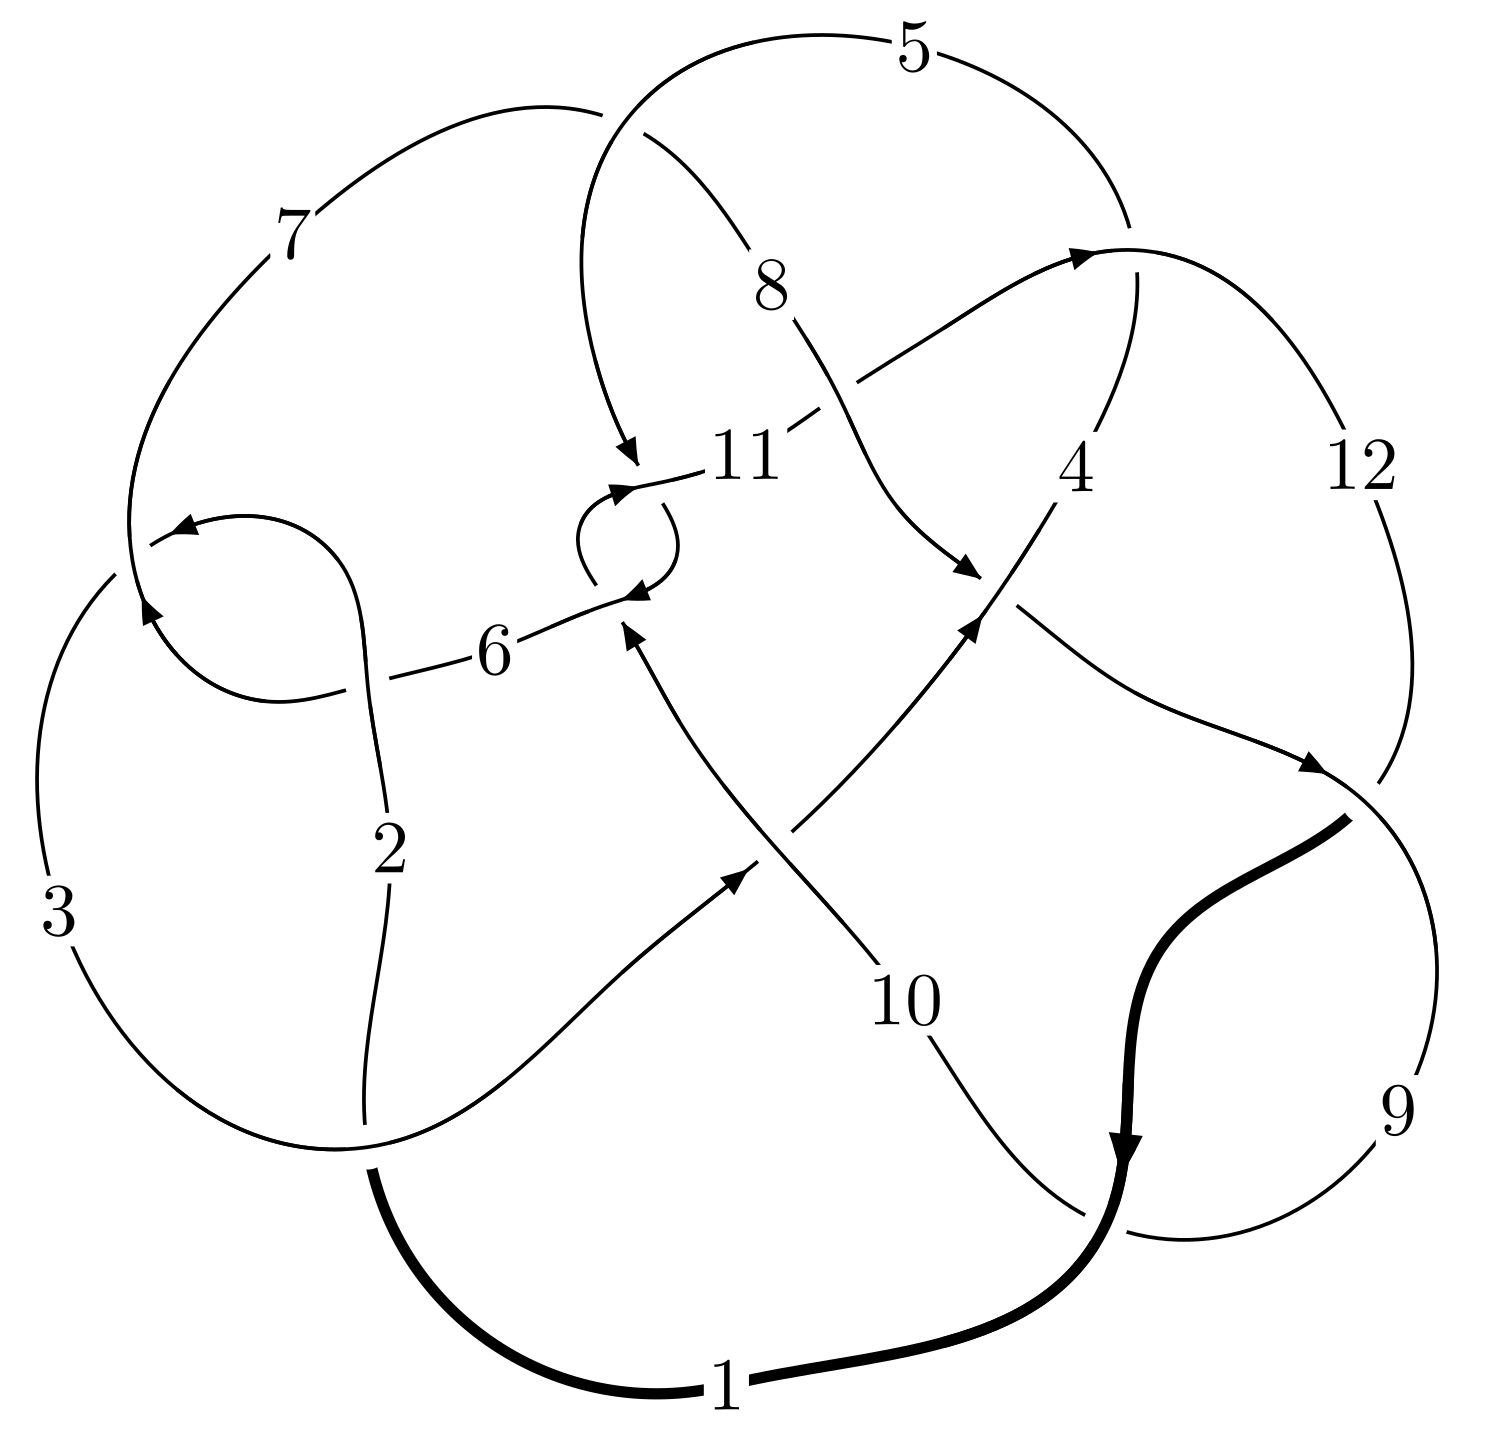
\includegraphics[width=112pt]{../../../GIT/diagram.site/Diagrams/png/1463_12a_0662.png}\\
\ \ \ A knot diagram\footnotemark}&
\allowdisplaybreaks
\textbf{Linearized knot diagam} \\
\cline{2-2}
 &
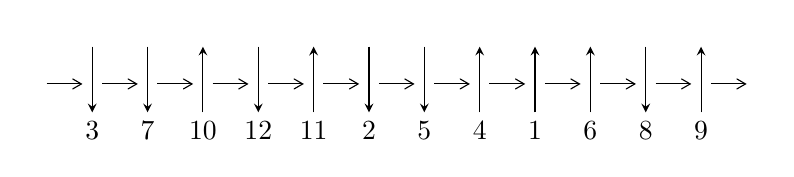
\begin{tikzpicture}[x=20pt, y=17pt]
	% nodes
	\node (C0) at (0, 0) {};
	\node (C1) at (1, 0) {};
	\node (C1U) at (1, +1) {};
	\node (C1D) at (1, -1) {3};

	\node (C2) at (2, 0) {};
	\node (C2U) at (2, +1) {};
	\node (C2D) at (2, -1) {7};

	\node (C3) at (3, 0) {};
	\node (C3U) at (3, +1) {};
	\node (C3D) at (3, -1) {10};

	\node (C4) at (4, 0) {};
	\node (C4U) at (4, +1) {};
	\node (C4D) at (4, -1) {12};

	\node (C5) at (5, 0) {};
	\node (C5U) at (5, +1) {};
	\node (C5D) at (5, -1) {11};

	\node (C6) at (6, 0) {};
	\node (C6U) at (6, +1) {};
	\node (C6D) at (6, -1) {2};

	\node (C7) at (7, 0) {};
	\node (C7U) at (7, +1) {};
	\node (C7D) at (7, -1) {5};

	\node (C8) at (8, 0) {};
	\node (C8U) at (8, +1) {};
	\node (C8D) at (8, -1) {4};

	\node (C9) at (9, 0) {};
	\node (C9U) at (9, +1) {};
	\node (C9D) at (9, -1) {1};

	\node (C10) at (10, 0) {};
	\node (C10U) at (10, +1) {};
	\node (C10D) at (10, -1) {6};

	\node (C11) at (11, 0) {};
	\node (C11U) at (11, +1) {};
	\node (C11D) at (11, -1) {8};

	\node (C12) at (12, 0) {};
	\node (C12U) at (12, +1) {};
	\node (C12D) at (12, -1) {9};
	\node (C13) at (13, 0) {};

	% arrows
	\draw[->,>={angle 60}]
	(C0) edge (C1) (C1) edge (C2) (C2) edge (C3) (C3) edge (C4) (C4) edge (C5) (C5) edge (C6) (C6) edge (C7) (C7) edge (C8) (C8) edge (C9) (C9) edge (C10) (C10) edge (C11) (C11) edge (C12) (C12) edge (C13) ;	\draw[->,>=stealth]
	(C1U) edge (C1D) (C2U) edge (C2D) (C3D) edge (C3U) (C4U) edge (C4D) (C5D) edge (C5U) (C6U) edge (C6D) (C7U) edge (C7D) (C8D) edge (C8U) (C9D) edge (C9U) (C10D) edge (C10U) (C11U) edge (C11D) (C12D) edge (C12U) ;
	\end{tikzpicture} \\
\hhline{~~} \\& 
\textbf{Solving Sequence} \\ \cline{2-2} 
 &
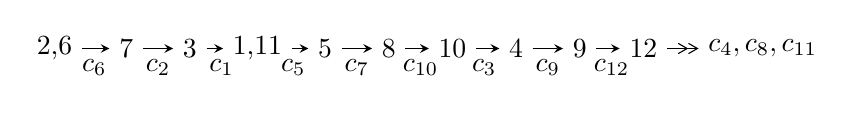
\begin{tikzpicture}[x=23pt, y=7pt]
	% node
	\node (A0) at (-1/8, 0) {2,6};
	\node (A1) at (1, 0) {7};
	\node (A2) at (2, 0) {3};
	\node (A3) at (49/16, 0) {1,11};
	\node (A4) at (33/8, 0) {5};
	\node (A5) at (41/8, 0) {8};
	\node (A6) at (49/8, 0) {10};
	\node (A7) at (57/8, 0) {4};
	\node (A8) at (65/8, 0) {9};
	\node (A9) at (73/8, 0) {12};
	\node (C1) at (1/2, -1) {$c_{6}$};
	\node (C2) at (3/2, -1) {$c_{2}$};
	\node (C3) at (5/2, -1) {$c_{1}$};
	\node (C4) at (29/8, -1) {$c_{5}$};
	\node (C5) at (37/8, -1) {$c_{7}$};
	\node (C6) at (45/8, -1) {$c_{10}$};
	\node (C7) at (53/8, -1) {$c_{3}$};
	\node (C8) at (61/8, -1) {$c_{9}$};
	\node (C9) at (69/8, -1) {$c_{12}$};
	\node (A10) at (11, 0) {$c_{4},c_{8},c_{11}$};

	% edge
	\draw[->,>=stealth]	
	(A0) edge (A1) (A1) edge (A2) (A2) edge (A3) (A3) edge (A4) (A4) edge (A5) (A5) edge (A6) (A6) edge (A7) (A7) edge (A8) (A8) edge (A9) ;
	\draw[->>,>={angle 60}]	
	(A9) edge (A10);
\end{tikzpicture} \\ 

\end{tabular} \\

\footnotetext{
The image of knot diagram is generated by the software ``\textbf{Draw programme}" developed by Andrew Bartholomew(\url{http://www.layer8.co.uk/maths/draw/index.htm\#Running-draw}), where we modified some parts for our purpose(\url{https://github.com/CATsTAILs/LinksPainter}).
}\phantom \\ \newline 
\centering \textbf{Ideals for irreducible components\footnotemark of $X_{\text{par}}$} 
 
\begin{align*}
I^u_{1}&=\langle 
-1.04261\times10^{439} u^{151}-3.12955\times10^{439} u^{150}+\cdots+2.44939\times10^{439} b+4.79597\times10^{441},\\
\phantom{I^u_{1}}&\phantom{= \langle  }-1.78662\times10^{442} u^{151}-2.88167\times10^{442} u^{150}+\cdots+8.98925\times10^{441} a+2.77990\times10^{444},\\
\phantom{I^u_{1}}&\phantom{= \langle  }u^{152}+u^{151}+\cdots-1379 u+367\rangle \\
I^u_{2}&=\langle 
-26479 u^{31}+2745 u^{30}+\cdots+5497 b-38311,\\
\phantom{I^u_{2}}&\phantom{= \langle  }-1129966 u^{31}+188660 u^{30}+\cdots+159413 a-2101975,\;u^{32}-8 u^{30}+\cdots+3 u+1\rangle \\
\\
\end{align*}
\raggedright * 2 irreducible components of $\dim_{\mathbb{C}}=0$, with total 184 representations.\\
\footnotetext{All coefficients of polynomials are rational numbers. But the coefficients are sometimes approximated in decimal forms when there is not enough margin.}
\newpage
\renewcommand{\arraystretch}{1}
\centering \section*{I. $I^u_{1}= \langle -1.04\times10^{439} u^{151}-3.13\times10^{439} u^{150}+\cdots+2.45\times10^{439} b+4.80\times10^{441},\;-1.79\times10^{442} u^{151}-2.88\times10^{442} u^{150}+\cdots+8.99\times10^{441} a+2.78\times10^{444},\;u^{152}+u^{151}+\cdots-1379 u+367 \rangle$}
\flushleft \textbf{(i) Arc colorings}\\
\begin{tabular}{m{7pt} m{180pt} m{7pt} m{180pt} }
\flushright $a_{2}=$&$\begin{pmatrix}0\\u\end{pmatrix}$ \\
\flushright $a_{6}=$&$\begin{pmatrix}1\\0\end{pmatrix}$ \\
\flushright $a_{7}=$&$\begin{pmatrix}1\\u^2\end{pmatrix}$ \\
\flushright $a_{3}=$&$\begin{pmatrix}- u\\- u^3+u\end{pmatrix}$ \\
\flushright $a_{1}=$&$\begin{pmatrix}u^3\\u^5- u^3+u\end{pmatrix}$ \\
\flushright $a_{11}=$&$\begin{pmatrix}1.98751 u^{151}+3.20568 u^{150}+\cdots+893.382 u-309.247\\0.425661 u^{151}+1.27769 u^{150}+\cdots+879.144 u-195.803\end{pmatrix}$ \\
\flushright $a_{5}=$&$\begin{pmatrix}-2.24943 u^{151}-3.02574 u^{150}+\cdots-2033.70 u+757.468\\2.06070 u^{151}+3.85778 u^{150}+\cdots+748.892 u-227.347\end{pmatrix}$ \\
\flushright $a_{8}=$&$\begin{pmatrix}-0.362640 u^{151}+1.75754 u^{150}+\cdots-1835.38 u+869.212\\-1.07197 u^{151}-1.99089 u^{150}+\cdots-638.367 u+196.579\end{pmatrix}$ \\
\flushright $a_{10}=$&$\begin{pmatrix}1.56185 u^{151}+1.92800 u^{150}+\cdots+14.2386 u-113.444\\0.425661 u^{151}+1.27769 u^{150}+\cdots+879.144 u-195.803\end{pmatrix}$ \\
\flushright $a_{4}=$&$\begin{pmatrix}-4.72164 u^{151}-10.0286 u^{150}+\cdots-5128.46 u+1430.34\\-2.42859 u^{151}-5.41972 u^{150}+\cdots-2029.05 u+490.243\end{pmatrix}$ \\
\flushright $a_{9}=$&$\begin{pmatrix}2.83491 u^{151}+4.20931 u^{150}+\cdots+917.177 u-418.112\\0.252785 u^{151}+0.661844 u^{150}+\cdots+229.065 u-46.6930\end{pmatrix}$ \\
\flushright $a_{12}=$&$\begin{pmatrix}1.76807 u^{151}+5.52351 u^{150}+\cdots-1817.01 u+740.392\\0.240114 u^{151}+0.0307253 u^{150}+\cdots+1184.40 u-370.130\end{pmatrix}$\\&\end{tabular}
\flushleft \textbf{(ii) Obstruction class $= -1$}\\~\\
\flushleft \textbf{(iii) Cusp Shapes $= -9.05646 u^{151}-13.2640 u^{150}+\cdots+563.221 u+212.918$}\\~\\
\newpage\renewcommand{\arraystretch}{1}
\flushleft \textbf{(iv) u-Polynomials at the component}\newline \\
\begin{tabular}{m{50pt}|m{274pt}}
Crossings & \hspace{64pt}u-Polynomials at each crossing \\
\hline $$\begin{aligned}c_{1}\end{aligned}$$&$\begin{aligned}
&u^{152}+63 u^{151}+\cdots+4922785 u+134689
\end{aligned}$\\
\hline $$\begin{aligned}c_{2},c_{6}\end{aligned}$$&$\begin{aligned}
&u^{152}- u^{151}+\cdots+1379 u+367
\end{aligned}$\\
\hline $$\begin{aligned}c_{3}\end{aligned}$$&$\begin{aligned}
&u^{152}+u^{151}+\cdots+589492 u+19909
\end{aligned}$\\
\hline $$\begin{aligned}c_{4}\end{aligned}$$&$\begin{aligned}
&u^{152}+4 u^{151}+\cdots+5694 u+7057
\end{aligned}$\\
\hline $$\begin{aligned}c_{5},c_{10}\end{aligned}$$&$\begin{aligned}
&u^{152}+u^{151}+\cdots-226661 u+18163
\end{aligned}$\\
\hline $$\begin{aligned}c_{7}\end{aligned}$$&$\begin{aligned}
&u^{152}-9 u^{151}+\cdots-50 u+1
\end{aligned}$\\
\hline $$\begin{aligned}c_{8}\end{aligned}$$&$\begin{aligned}
&u^{152}-4 u^{151}+\cdots+22 u+1
\end{aligned}$\\
\hline $$\begin{aligned}c_{9},c_{12}\end{aligned}$$&$\begin{aligned}
&u^{152}-3 u^{151}+\cdots-2650 u+223
\end{aligned}$\\
\hline $$\begin{aligned}c_{11}\end{aligned}$$&$\begin{aligned}
&u^{152}+7 u^{151}+\cdots+59968 u+7903
\end{aligned}$\\
\hline
\end{tabular}\\~\\
\newpage\renewcommand{\arraystretch}{1}
\flushleft \textbf{(v) Riley Polynomials at the component}\newline \\
\begin{tabular}{m{50pt}|m{274pt}}
Crossings & \hspace{64pt}Riley Polynomials at each crossing \\
\hline $$\begin{aligned}c_{1}\end{aligned}$$&$\begin{aligned}
&y^{152}+61 y^{151}+\cdots+143171208307 y+18141126721
\end{aligned}$\\
\hline $$\begin{aligned}c_{2},c_{6}\end{aligned}$$&$\begin{aligned}
&y^{152}-63 y^{151}+\cdots-4922785 y+134689
\end{aligned}$\\
\hline $$\begin{aligned}c_{3}\end{aligned}$$&$\begin{aligned}
&y^{152}-27 y^{151}+\cdots-116608221282 y+396368281
\end{aligned}$\\
\hline $$\begin{aligned}c_{4}\end{aligned}$$&$\begin{aligned}
&y^{152}+38 y^{151}+\cdots+3402431974 y+49801249
\end{aligned}$\\
\hline $$\begin{aligned}c_{5},c_{10}\end{aligned}$$&$\begin{aligned}
&y^{152}+105 y^{151}+\cdots-5729591991 y+329894569
\end{aligned}$\\
\hline $$\begin{aligned}c_{7}\end{aligned}$$&$\begin{aligned}
&y^{152}-5 y^{151}+\cdots-68 y+1
\end{aligned}$\\
\hline $$\begin{aligned}c_{8}\end{aligned}$$&$\begin{aligned}
&y^{152}-8 y^{151}+\cdots-22 y+1
\end{aligned}$\\
\hline $$\begin{aligned}c_{9},c_{12}\end{aligned}$$&$\begin{aligned}
&y^{152}-119 y^{151}+\cdots-2364476 y+49729
\end{aligned}$\\
\hline $$\begin{aligned}c_{11}\end{aligned}$$&$\begin{aligned}
&y^{152}-39 y^{151}+\cdots-5965053662 y+62457409
\end{aligned}$\\
\hline
\end{tabular}\\~\\
\newpage\flushleft \textbf{(vi) Complex Volumes and Cusp Shapes}
$$\begin{array}{c|c|c}  
\text{Solutions to }I^u_{1}& \I (\text{vol} + \sqrt{-1}CS) & \text{Cusp shape}\\
 \hline 
\begin{aligned}
u &= -0.976618 + 0.216947 I \\
a &= -0.10966 - 2.80122 I \\
b &= \phantom{-}0.02771 - 1.44061 I\end{aligned}
 & -7.74674 + 0.74291 I & \phantom{-0.000000 } 0 \\ \hline\begin{aligned}
u &= -0.976618 - 0.216947 I \\
a &= -0.10966 + 2.80122 I \\
b &= \phantom{-}0.02771 + 1.44061 I\end{aligned}
 & -7.74674 - 0.74291 I & \phantom{-0.000000 } 0 \\ \hline\begin{aligned}
u &= -0.865113 + 0.510791 I \\
a &= -0.91463 + 2.22114 I \\
b &= -0.08851 + 1.63090 I\end{aligned}
 & -1.47039 + 2.06741 I & \phantom{-0.000000 } 0 \\ \hline\begin{aligned}
u &= -0.865113 - 0.510791 I \\
a &= -0.91463 - 2.22114 I \\
b &= -0.08851 - 1.63090 I\end{aligned}
 & -1.47039 - 2.06741 I & \phantom{-0.000000 } 0 \\ \hline\begin{aligned}
u &= \phantom{-}0.572612 + 0.830099 I \\
a &= \phantom{-}0.342921 - 0.154395 I \\
b &= -0.540329 - 1.235470 I\end{aligned}
 & -0.28796 + 5.49864 I & \phantom{-0.000000 } 0 \\ \hline\begin{aligned}
u &= \phantom{-}0.572612 - 0.830099 I \\
a &= \phantom{-}0.342921 + 0.154395 I \\
b &= -0.540329 + 1.235470 I\end{aligned}
 & -0.28796 - 5.49864 I & \phantom{-0.000000 } 0 \\ \hline\begin{aligned}
u &= -0.804913 + 0.577587 I \\
a &= \phantom{-}1.36576 - 1.94031 I \\
b &= -1.00500 - 1.39736 I\end{aligned}
 & \phantom{-}2.90265 - 0.91653 I & \phantom{-0.000000 } 0 \\ \hline\begin{aligned}
u &= -0.804913 - 0.577587 I \\
a &= \phantom{-}1.36576 + 1.94031 I \\
b &= -1.00500 + 1.39736 I\end{aligned}
 & \phantom{-}2.90265 + 0.91653 I & \phantom{-0.000000 } 0 \\ \hline\begin{aligned}
u &= -1.007170 + 0.071305 I \\
a &= -0.66068 + 2.50970 I \\
b &= -0.16176 + 1.55220 I\end{aligned}
 & -8.06070 - 0.34368 I & \phantom{-0.000000 } 0 \\ \hline\begin{aligned}
u &= -1.007170 - 0.071305 I \\
a &= -0.66068 - 2.50970 I \\
b &= -0.16176 - 1.55220 I\end{aligned}
 & -8.06070 + 0.34368 I & \phantom{-0.000000 } 0\\
 \hline 
 \end{array}$$\newpage$$\begin{array}{c|c|c}  
\text{Solutions to }I^u_{1}& \I (\text{vol} + \sqrt{-1}CS) & \text{Cusp shape}\\
 \hline 
\begin{aligned}
u &= \phantom{-}0.862567 + 0.483048 I \\
a &= \phantom{-}1.66883 + 0.68631 I \\
b &= -0.224587 + 1.223930 I\end{aligned}
 & -1.62821 - 1.97022 I & \phantom{-0.000000 } 0 \\ \hline\begin{aligned}
u &= \phantom{-}0.862567 - 0.483048 I \\
a &= \phantom{-}1.66883 - 0.68631 I \\
b &= -0.224587 - 1.223930 I\end{aligned}
 & -1.62821 + 1.97022 I & \phantom{-0.000000 } 0 \\ \hline\begin{aligned}
u &= -0.745359 + 0.636841 I \\
a &= \phantom{-}0.502927 - 0.311138 I \\
b &= -0.772595 - 0.278417 I\end{aligned}
 & \phantom{-}2.57935 + 0.80193 I & \phantom{-0.000000 } 0 \\ \hline\begin{aligned}
u &= -0.745359 - 0.636841 I \\
a &= \phantom{-}0.502927 + 0.311138 I \\
b &= -0.772595 + 0.278417 I\end{aligned}
 & \phantom{-}2.57935 - 0.80193 I & \phantom{-0.000000 } 0 \\ \hline\begin{aligned}
u &= \phantom{-}0.851678 + 0.564295 I \\
a &= -0.740309 + 0.501044 I \\
b &= \phantom{-}0.530138 + 1.114300 I\end{aligned}
 & \phantom{-}2.45684 + 3.76901 I & \phantom{-0.000000 } 0 \\ \hline\begin{aligned}
u &= \phantom{-}0.851678 - 0.564295 I \\
a &= -0.740309 - 0.501044 I \\
b &= \phantom{-}0.530138 - 1.114300 I\end{aligned}
 & \phantom{-}2.45684 - 3.76901 I & \phantom{-0.000000 } 0 \\ \hline\begin{aligned}
u &= -0.919952 + 0.329313 I \\
a &= -1.173450 - 0.011749 I \\
b &= \phantom{-}0.100577 - 0.324560 I\end{aligned}
 & -2.58832 + 3.84915 I & \phantom{-0.000000 } 0 \\ \hline\begin{aligned}
u &= -0.919952 - 0.329313 I \\
a &= -1.173450 + 0.011749 I \\
b &= \phantom{-}0.100577 + 0.324560 I\end{aligned}
 & -2.58832 - 3.84915 I & \phantom{-0.000000 } 0 \\ \hline\begin{aligned}
u &= \phantom{-}0.864184 + 0.552906 I \\
a &= \phantom{-}2.26119 + 2.71298 I \\
b &= -0.379127 + 1.199260 I\end{aligned}
 & \phantom{-}2.42176 - 8.23014 I & \phantom{-0.000000 } 0 \\ \hline\begin{aligned}
u &= \phantom{-}0.864184 - 0.552906 I \\
a &= \phantom{-}2.26119 - 2.71298 I \\
b &= -0.379127 - 1.199260 I\end{aligned}
 & \phantom{-}2.42176 + 8.23014 I & \phantom{-0.000000 } 0\\
 \hline 
 \end{array}$$\newpage$$\begin{array}{c|c|c}  
\text{Solutions to }I^u_{1}& \I (\text{vol} + \sqrt{-1}CS) & \text{Cusp shape}\\
 \hline 
\begin{aligned}
u &= \phantom{-}0.849802 + 0.580022 I \\
a &= -1.25646 - 2.10652 I \\
b &= \phantom{-}0.180753 - 1.091820 I\end{aligned}
 & \phantom{-}3.69053 - 3.19749 I & \phantom{-0.000000 } 0 \\ \hline\begin{aligned}
u &= \phantom{-}0.849802 - 0.580022 I \\
a &= -1.25646 + 2.10652 I \\
b &= \phantom{-}0.180753 + 1.091820 I\end{aligned}
 & \phantom{-}3.69053 + 3.19749 I & \phantom{-0.000000 } 0 \\ \hline\begin{aligned}
u &= \phantom{-}0.850752 + 0.584637 I \\
a &= \phantom{-}0.074575 - 1.074680 I \\
b &= -0.449062 - 0.991318 I\end{aligned}
 & \phantom{-}3.68435 - 1.42902 I & \phantom{-0.000000 } 0 \\ \hline\begin{aligned}
u &= \phantom{-}0.850752 - 0.584637 I \\
a &= \phantom{-}0.074575 + 1.074680 I \\
b &= -0.449062 + 0.991318 I\end{aligned}
 & \phantom{-}3.68435 + 1.42902 I & \phantom{-0.000000 } 0 \\ \hline\begin{aligned}
u &= \phantom{-}0.639559 + 0.812305 I \\
a &= \phantom{-}0.277848 + 0.749378 I \\
b &= -1.131630 - 0.010331 I\end{aligned}
 & \phantom{-}7.08155 + 7.79782 I & \phantom{-0.000000 } 0 \\ \hline\begin{aligned}
u &= \phantom{-}0.639559 - 0.812305 I \\
a &= \phantom{-}0.277848 - 0.749378 I \\
b &= -1.131630 + 0.010331 I\end{aligned}
 & \phantom{-}7.08155 - 7.79782 I & \phantom{-0.000000 } 0 \\ \hline\begin{aligned}
u &= -0.950501 + 0.161280 I \\
a &= \phantom{-}0.455484 + 0.011996 I \\
b &= \phantom{-}0.708579 + 0.554908 I\end{aligned}
 & \phantom{-}0.83341 + 7.86376 I & \phantom{-0.000000 } 0 \\ \hline\begin{aligned}
u &= -0.950501 - 0.161280 I \\
a &= \phantom{-}0.455484 - 0.011996 I \\
b &= \phantom{-}0.708579 - 0.554908 I\end{aligned}
 & \phantom{-}0.83341 - 7.86376 I & \phantom{-0.000000 } 0 \\ \hline\begin{aligned}
u &= \phantom{-}0.660685 + 0.804281 I \\
a &= -0.460261 - 0.955987 I \\
b &= \phantom{-}0.803987 - 0.508923 I\end{aligned}
 & \phantom{-}7.04453 + 0.84251 I & \phantom{-0.000000 } 0 \\ \hline\begin{aligned}
u &= \phantom{-}0.660685 - 0.804281 I \\
a &= -0.460261 + 0.955987 I \\
b &= \phantom{-}0.803987 + 0.508923 I\end{aligned}
 & \phantom{-}7.04453 - 0.84251 I & \phantom{-0.000000 } 0\\
 \hline 
 \end{array}$$\newpage$$\begin{array}{c|c|c}  
\text{Solutions to }I^u_{1}& \I (\text{vol} + \sqrt{-1}CS) & \text{Cusp shape}\\
 \hline 
\begin{aligned}
u &= \phantom{-}0.950182 + 0.465480 I \\
a &= \phantom{-}0.094286 + 0.516746 I \\
b &= \phantom{-}0.296626 + 0.481035 I\end{aligned}
 & -1.71761 - 1.68861 I & \phantom{-0.000000 } 0 \\ \hline\begin{aligned}
u &= \phantom{-}0.950182 - 0.465480 I \\
a &= \phantom{-}0.094286 - 0.516746 I \\
b &= \phantom{-}0.296626 - 0.481035 I\end{aligned}
 & -1.71761 + 1.68861 I & \phantom{-0.000000 } 0 \\ \hline\begin{aligned}
u &= -0.406856 + 0.845498 I \\
a &= -0.032963 - 0.295662 I \\
b &= \phantom{-}0.56540 - 1.31168 I\end{aligned}
 & -2.50384 - 8.49483 I & \phantom{-0.000000 } 0 \\ \hline\begin{aligned}
u &= -0.406856 - 0.845498 I \\
a &= -0.032963 + 0.295662 I \\
b &= \phantom{-}0.56540 + 1.31168 I\end{aligned}
 & -2.50384 + 8.49483 I & \phantom{-0.000000 } 0 \\ \hline\begin{aligned}
u &= -0.887774 + 0.582678 I \\
a &= \phantom{-}0.935153 + 0.083120 I \\
b &= \phantom{-}1.22014 - 1.26923 I\end{aligned}
 & \phantom{-}2.63555 + 5.53579 I & \phantom{-0.000000 } 0 \\ \hline\begin{aligned}
u &= -0.887774 - 0.582678 I \\
a &= \phantom{-}0.935153 - 0.083120 I \\
b &= \phantom{-}1.22014 + 1.26923 I\end{aligned}
 & \phantom{-}2.63555 - 5.53579 I & \phantom{-0.000000 } 0 \\ \hline\begin{aligned}
u &= -0.818657 + 0.450572 I \\
a &= -3.28553 + 1.87639 I \\
b &= -0.059830 + 0.982360 I\end{aligned}
 & \phantom{-}1.74623 - 4.46561 I & \phantom{-0.000000 } 0 \\ \hline\begin{aligned}
u &= -0.818657 - 0.450572 I \\
a &= -3.28553 - 1.87639 I \\
b &= -0.059830 - 0.982360 I\end{aligned}
 & \phantom{-}1.74623 + 4.46561 I & \phantom{-0.000000 } 0 \\ \hline\begin{aligned}
u &= \phantom{-}0.823901 + 0.681823 I \\
a &= -1.19203 - 1.20702 I \\
b &= -0.12432 - 1.63512 I\end{aligned}
 & \phantom{-}2.85259 - 2.62751 I & \phantom{-0.000000 } 0 \\ \hline\begin{aligned}
u &= \phantom{-}0.823901 - 0.681823 I \\
a &= -1.19203 + 1.20702 I \\
b &= -0.12432 + 1.63512 I\end{aligned}
 & \phantom{-}2.85259 + 2.62751 I & \phantom{-0.000000 } 0\\
 \hline 
 \end{array}$$\newpage$$\begin{array}{c|c|c}  
\text{Solutions to }I^u_{1}& \I (\text{vol} + \sqrt{-1}CS) & \text{Cusp shape}\\
 \hline 
\begin{aligned}
u &= \phantom{-}0.926283\phantom{ +0.000000I} \\
a &= \phantom{-}0.854247\phantom{ +0.000000I} \\
b &= \phantom{-}0.760609\phantom{ +0.000000I}\end{aligned}
 & -1.61290\phantom{ +0.000000I} & \phantom{-0.000000 } 0 \\ \hline\begin{aligned}
u &= -0.977472 + 0.473192 I \\
a &= \phantom{-}0.938151 - 0.165156 I \\
b &= -0.011295 + 0.587086 I\end{aligned}
 & \phantom{-}1.20459 + 8.18013 I & \phantom{-0.000000 } 0 \\ \hline\begin{aligned}
u &= -0.977472 - 0.473192 I \\
a &= \phantom{-}0.938151 + 0.165156 I \\
b &= -0.011295 - 0.587086 I\end{aligned}
 & \phantom{-}1.20459 - 8.18013 I & \phantom{-0.000000 } 0 \\ \hline\begin{aligned}
u &= -0.649188 + 0.876413 I \\
a &= -0.238761 + 0.471482 I \\
b &= \phantom{-}0.736869 + 0.099610 I\end{aligned}
 & \phantom{-}7.68334 + 0.25660 I & \phantom{-0.000000 } 0 \\ \hline\begin{aligned}
u &= -0.649188 - 0.876413 I \\
a &= -0.238761 - 0.471482 I \\
b &= \phantom{-}0.736869 - 0.099610 I\end{aligned}
 & \phantom{-}7.68334 - 0.25660 I & \phantom{-0.000000 } 0 \\ \hline\begin{aligned}
u &= -0.805819 + 0.748960 I \\
a &= \phantom{-}0.105328 - 1.206030 I \\
b &= -0.634172 + 0.360662 I\end{aligned}
 & \phantom{-}5.12004 + 4.30665 I & \phantom{-0.000000 } 0 \\ \hline\begin{aligned}
u &= -0.805819 - 0.748960 I \\
a &= \phantom{-}0.105328 + 1.206030 I \\
b &= -0.634172 - 0.360662 I\end{aligned}
 & \phantom{-}5.12004 - 4.30665 I & \phantom{-0.000000 } 0 \\ \hline\begin{aligned}
u &= \phantom{-}0.939555 + 0.575189 I \\
a &= -0.274937 + 1.214310 I \\
b &= -1.53346 + 0.18549 I\end{aligned}
 & \phantom{-}0.35184 - 6.84298 I & \phantom{-0.000000 } 0 \\ \hline\begin{aligned}
u &= \phantom{-}0.939555 - 0.575189 I \\
a &= -0.274937 - 1.214310 I \\
b &= -1.53346 - 0.18549 I\end{aligned}
 & \phantom{-}0.35184 + 6.84298 I & \phantom{-0.000000 } 0 \\ \hline\begin{aligned}
u &= \phantom{-}0.458825 + 0.763650 I \\
a &= -1.047300 + 0.514506 I \\
b &= \phantom{-}0.037737 + 1.087970 I\end{aligned}
 & \phantom{-}1.08065 + 4.08048 I & \phantom{-0.000000 } 0\\
 \hline 
 \end{array}$$\newpage$$\begin{array}{c|c|c}  
\text{Solutions to }I^u_{1}& \I (\text{vol} + \sqrt{-1}CS) & \text{Cusp shape}\\
 \hline 
\begin{aligned}
u &= \phantom{-}0.458825 - 0.763650 I \\
a &= -1.047300 - 0.514506 I \\
b &= \phantom{-}0.037737 - 1.087970 I\end{aligned}
 & \phantom{-}1.08065 - 4.08048 I & \phantom{-0.000000 } 0 \\ \hline\begin{aligned}
u &= \phantom{-}0.539514 + 0.699005 I \\
a &= \phantom{-}0.206542 - 0.079255 I \\
b &= \phantom{-}0.536198 + 1.293110 I\end{aligned}
 & -3.17732 + 1.39405 I & \phantom{-0.000000 } 0 \\ \hline\begin{aligned}
u &= \phantom{-}0.539514 - 0.699005 I \\
a &= \phantom{-}0.206542 + 0.079255 I \\
b &= \phantom{-}0.536198 - 1.293110 I\end{aligned}
 & -3.17732 - 1.39405 I & \phantom{-0.000000 } 0 \\ \hline\begin{aligned}
u &= \phantom{-}0.703112 + 0.534095 I \\
a &= -0.071455 - 1.308950 I \\
b &= \phantom{-}1.344760 - 0.215123 I\end{aligned}
 & \phantom{-}1.08035 + 2.31080 I & \phantom{-0.000000 } 0 \\ \hline\begin{aligned}
u &= \phantom{-}0.703112 - 0.534095 I \\
a &= -0.071455 + 1.308950 I \\
b &= \phantom{-}1.344760 + 0.215123 I\end{aligned}
 & \phantom{-}1.08035 - 2.31080 I & \phantom{-0.000000 } 0 \\ \hline\begin{aligned}
u &= -0.537922 + 0.983429 I \\
a &= \phantom{-}0.048509 + 0.489775 I \\
b &= -0.54128 + 1.35705 I\end{aligned}
 & \phantom{-}2.81822 - 13.64750 I & \phantom{-0.000000 } 0 \\ \hline\begin{aligned}
u &= -0.537922 - 0.983429 I \\
a &= \phantom{-}0.048509 - 0.489775 I \\
b &= -0.54128 - 1.35705 I\end{aligned}
 & \phantom{-}2.81822 + 13.64750 I & \phantom{-0.000000 } 0 \\ \hline\begin{aligned}
u &= \phantom{-}0.878444\phantom{ +0.000000I} \\
a &= \phantom{-}0.765301\phantom{ +0.000000I} \\
b &= \phantom{-}0.512720\phantom{ +0.000000I}\end{aligned}
 & -1.64970\phantom{ +0.000000I} & \phantom{-0.000000 } 0 \\ \hline\begin{aligned}
u &= -1.009080 + 0.491975 I \\
a &= -1.03079 + 2.15983 I \\
b &= \phantom{-}0.87359 + 1.38392 I\end{aligned}
 & -2.60289 + 6.20359 I & \phantom{-0.000000 } 0 \\ \hline\begin{aligned}
u &= -1.009080 - 0.491975 I \\
a &= -1.03079 - 2.15983 I \\
b &= \phantom{-}0.87359 - 1.38392 I\end{aligned}
 & -2.60289 - 6.20359 I & \phantom{-0.000000 } 0\\
 \hline 
 \end{array}$$\newpage$$\begin{array}{c|c|c}  
\text{Solutions to }I^u_{1}& \I (\text{vol} + \sqrt{-1}CS) & \text{Cusp shape}\\
 \hline 
\begin{aligned}
u &= \phantom{-}0.427475 + 1.040220 I \\
a &= -0.056678 + 0.787178 I \\
b &= \phantom{-}0.372426 + 1.198790 I\end{aligned}
 & \phantom{-}4.32849 + 3.82697 I & \phantom{-0.000000 } 0 \\ \hline\begin{aligned}
u &= \phantom{-}0.427475 - 1.040220 I \\
a &= -0.056678 - 0.787178 I \\
b &= \phantom{-}0.372426 - 1.198790 I\end{aligned}
 & \phantom{-}4.32849 - 3.82697 I & \phantom{-0.000000 } 0 \\ \hline\begin{aligned}
u &= -0.918955 + 0.650665 I \\
a &= \phantom{-}0.077171 + 0.811335 I \\
b &= \phantom{-}0.754789 - 0.079899 I\end{aligned}
 & \phantom{-}2.06466 + 4.23388 I & \phantom{-0.000000 } 0 \\ \hline\begin{aligned}
u &= -0.918955 - 0.650665 I \\
a &= \phantom{-}0.077171 - 0.811335 I \\
b &= \phantom{-}0.754789 + 0.079899 I\end{aligned}
 & \phantom{-}2.06466 - 4.23388 I & \phantom{-0.000000 } 0 \\ \hline\begin{aligned}
u &= \phantom{-}1.063870 + 0.369962 I \\
a &= \phantom{-}1.31086 + 1.33153 I \\
b &= \phantom{-}0.42212 + 1.42825 I\end{aligned}
 & -3.28779 - 0.28143 I & \phantom{-0.000000 } 0 \\ \hline\begin{aligned}
u &= \phantom{-}1.063870 - 0.369962 I \\
a &= \phantom{-}1.31086 - 1.33153 I \\
b &= \phantom{-}0.42212 - 1.42825 I\end{aligned}
 & -3.28779 + 0.28143 I & \phantom{-0.000000 } 0 \\ \hline\begin{aligned}
u &= -0.669425 + 0.556263 I \\
a &= \phantom{-}1.39519 - 0.74758 I \\
b &= -0.769467 - 0.429201 I\end{aligned}
 & \phantom{-}2.53454 - 0.28463 I & \phantom{-0.000000 } 0 \\ \hline\begin{aligned}
u &= -0.669425 - 0.556263 I \\
a &= \phantom{-}1.39519 + 0.74758 I \\
b &= -0.769467 + 0.429201 I\end{aligned}
 & \phantom{-}2.53454 + 0.28463 I & \phantom{-0.000000 } 0 \\ \hline\begin{aligned}
u &= -0.960743 + 0.609210 I \\
a &= \phantom{-}0.028076 + 0.866700 I \\
b &= \phantom{-}1.102640 - 0.252664 I\end{aligned}
 & \phantom{-}1.65873 + 5.03382 I & \phantom{-0.000000 } 0 \\ \hline\begin{aligned}
u &= -0.960743 - 0.609210 I \\
a &= \phantom{-}0.028076 - 0.866700 I \\
b &= \phantom{-}1.102640 + 0.252664 I\end{aligned}
 & \phantom{-}1.65873 - 5.03382 I & \phantom{-0.000000 } 0\\
 \hline 
 \end{array}$$\newpage$$\begin{array}{c|c|c}  
\text{Solutions to }I^u_{1}& \I (\text{vol} + \sqrt{-1}CS) & \text{Cusp shape}\\
 \hline 
\begin{aligned}
u &= -0.475350 + 1.035040 I \\
a &= -0.060496 - 0.461301 I \\
b &= \phantom{-}0.452078 - 0.961673 I\end{aligned}
 & \phantom{-}5.61630 - 5.52289 I & \phantom{-0.000000 } 0 \\ \hline\begin{aligned}
u &= -0.475350 - 1.035040 I \\
a &= -0.060496 + 0.461301 I \\
b &= \phantom{-}0.452078 + 0.961673 I\end{aligned}
 & \phantom{-}5.61630 + 5.52289 I & \phantom{-0.000000 } 0 \\ \hline\begin{aligned}
u &= -1.069980 + 0.399619 I \\
a &= \phantom{-}1.48760 - 1.98942 I \\
b &= \phantom{-}0.030102 - 1.047000 I\end{aligned}
 & -3.47061 - 1.39309 I & \phantom{-0.000000 } 0 \\ \hline\begin{aligned}
u &= -1.069980 - 0.399619 I \\
a &= \phantom{-}1.48760 + 1.98942 I \\
b &= \phantom{-}0.030102 + 1.047000 I\end{aligned}
 & -3.47061 + 1.39309 I & \phantom{-0.000000 } 0 \\ \hline\begin{aligned}
u &= \phantom{-}0.046085 + 0.855577 I \\
a &= -0.239658 - 0.787458 I \\
b &= -0.297747 - 0.177190 I\end{aligned}
 & \phantom{-}4.31998 - 4.77119 I & \phantom{-0.000000 } 0 \\ \hline\begin{aligned}
u &= \phantom{-}0.046085 - 0.855577 I \\
a &= -0.239658 + 0.787458 I \\
b &= -0.297747 + 0.177190 I\end{aligned}
 & \phantom{-}4.31998 + 4.77119 I & \phantom{-0.000000 } 0 \\ \hline\begin{aligned}
u &= -1.150540 + 0.033163 I \\
a &= \phantom{-}0.04175 + 2.34065 I \\
b &= \phantom{-}0.327382 + 1.370250 I\end{aligned}
 & -6.47670 + 4.16409 I & \phantom{-0.000000 } 0 \\ \hline\begin{aligned}
u &= -1.150540 - 0.033163 I \\
a &= \phantom{-}0.04175 - 2.34065 I \\
b &= \phantom{-}0.327382 - 1.370250 I\end{aligned}
 & -6.47670 - 4.16409 I & \phantom{-0.000000 } 0 \\ \hline\begin{aligned}
u &= -0.764698 + 0.354028 I \\
a &= -0.694778 - 0.393450 I \\
b &= -1.06922 + 0.98003 I\end{aligned}
 & -1.48089 - 2.58427 I & \phantom{-0.000000 } 0 \\ \hline\begin{aligned}
u &= -0.764698 - 0.354028 I \\
a &= -0.694778 + 0.393450 I \\
b &= -1.06922 - 0.98003 I\end{aligned}
 & -1.48089 + 2.58427 I & \phantom{-0.000000 } 0\\
 \hline 
 \end{array}$$\newpage$$\begin{array}{c|c|c}  
\text{Solutions to }I^u_{1}& \I (\text{vol} + \sqrt{-1}CS) & \text{Cusp shape}\\
 \hline 
\begin{aligned}
u &= -0.931412 + 0.706267 I \\
a &= -0.735829 + 0.157932 I \\
b &= \phantom{-}0.813993 + 0.382368 I\end{aligned}
 & \phantom{-}4.71540 + 1.23998 I & \phantom{-0.000000 } 0 \\ \hline\begin{aligned}
u &= -0.931412 - 0.706267 I \\
a &= -0.735829 - 0.157932 I \\
b &= \phantom{-}0.813993 - 0.382368 I\end{aligned}
 & \phantom{-}4.71540 - 1.23998 I & \phantom{-0.000000 } 0 \\ \hline\begin{aligned}
u &= \phantom{-}0.479078 + 0.677748 I \\
a &= \phantom{-}0.511177 + 0.249312 I \\
b &= -0.215463 + 1.061590 I\end{aligned}
 & -1.05102 - 2.47699 I & \phantom{-0.000000 } 0 \\ \hline\begin{aligned}
u &= \phantom{-}0.479078 - 0.677748 I \\
a &= \phantom{-}0.511177 - 0.249312 I \\
b &= -0.215463 - 1.061590 I\end{aligned}
 & -1.05102 + 2.47699 I & \phantom{-0.000000 } 0 \\ \hline\begin{aligned}
u &= \phantom{-}0.462726 + 0.668814 I \\
a &= \phantom{-}0.480800 + 0.040833 I \\
b &= \phantom{-}0.021718 - 1.074260 I\end{aligned}
 & -3.50685 + 0.66121 I & \phantom{-0.000000 } 0 \\ \hline\begin{aligned}
u &= \phantom{-}0.462726 - 0.668814 I \\
a &= \phantom{-}0.480800 - 0.040833 I \\
b &= \phantom{-}0.021718 + 1.074260 I\end{aligned}
 & -3.50685 - 0.66121 I & \phantom{-0.000000 } 0 \\ \hline\begin{aligned}
u &= \phantom{-}1.044590 + 0.583400 I \\
a &= -1.75741 - 1.11724 I \\
b &= \phantom{-}0.187605 - 1.144610 I\end{aligned}
 & -5.17008 - 5.51409 I & \phantom{-0.000000 } 0 \\ \hline\begin{aligned}
u &= \phantom{-}1.044590 - 0.583400 I \\
a &= -1.75741 + 1.11724 I \\
b &= \phantom{-}0.187605 + 1.144610 I\end{aligned}
 & -5.17008 + 5.51409 I & \phantom{-0.000000 } 0 \\ \hline\begin{aligned}
u &= -0.885638 + 0.811835 I \\
a &= \phantom{-}0.609964 + 0.376082 I \\
b &= -0.051715 - 0.915336 I\end{aligned}
 & \phantom{-}5.00003 + 3.02886 I & \phantom{-0.000000 } 0 \\ \hline\begin{aligned}
u &= -0.885638 - 0.811835 I \\
a &= \phantom{-}0.609964 - 0.376082 I \\
b &= -0.051715 + 0.915336 I\end{aligned}
 & \phantom{-}5.00003 - 3.02886 I & \phantom{-0.000000 } 0\\
 \hline 
 \end{array}$$\newpage$$\begin{array}{c|c|c}  
\text{Solutions to }I^u_{1}& \I (\text{vol} + \sqrt{-1}CS) & \text{Cusp shape}\\
 \hline 
\begin{aligned}
u &= \phantom{-}1.030060 + 0.623389 I \\
a &= \phantom{-}1.33548 + 1.65672 I \\
b &= -0.62080 + 1.50727 I\end{aligned}
 & -4.59816 - 6.49408 I & \phantom{-0.000000 } 0 \\ \hline\begin{aligned}
u &= \phantom{-}1.030060 - 0.623389 I \\
a &= \phantom{-}1.33548 - 1.65672 I \\
b &= -0.62080 - 1.50727 I\end{aligned}
 & -4.59816 + 6.49408 I & \phantom{-0.000000 } 0 \\ \hline\begin{aligned}
u &= \phantom{-}1.195750 + 0.212199 I \\
a &= \phantom{-}0.089352 - 0.369095 I \\
b &= -0.197353 - 0.034124 I\end{aligned}
 & \phantom{-}0.013101 + 0.934312 I & \phantom{-0.000000 } 0 \\ \hline\begin{aligned}
u &= \phantom{-}1.195750 - 0.212199 I \\
a &= \phantom{-}0.089352 + 0.369095 I \\
b &= -0.197353 + 0.034124 I\end{aligned}
 & \phantom{-}0.013101 - 0.934312 I & \phantom{-0.000000 } 0 \\ \hline\begin{aligned}
u &= \phantom{-}1.068640 + 0.581893 I \\
a &= -1.30648 - 2.15328 I \\
b &= \phantom{-}0.398500 - 1.302870 I\end{aligned}
 & -1.85136 - 8.54719 I & \phantom{-0.000000 } 0 \\ \hline\begin{aligned}
u &= \phantom{-}1.068640 - 0.581893 I \\
a &= -1.30648 + 2.15328 I \\
b &= \phantom{-}0.398500 + 1.302870 I\end{aligned}
 & -1.85136 + 8.54719 I & \phantom{-0.000000 } 0 \\ \hline\begin{aligned}
u &= -1.096240 + 0.528676 I \\
a &= -0.86983 + 1.69195 I \\
b &= \phantom{-}0.611574 + 0.963903 I\end{aligned}
 & -1.47654 + 5.76364 I & \phantom{-0.000000 } 0 \\ \hline\begin{aligned}
u &= -1.096240 - 0.528676 I \\
a &= -0.86983 - 1.69195 I \\
b &= \phantom{-}0.611574 - 0.963903 I\end{aligned}
 & -1.47654 - 5.76364 I & \phantom{-0.000000 } 0 \\ \hline\begin{aligned}
u &= -1.208030 + 0.158012 I \\
a &= \phantom{-}0.31166 + 2.70295 I \\
b &= -0.020873 + 1.299230 I\end{aligned}
 & -4.11234 - 1.67628 I & \phantom{-0.000000 } 0 \\ \hline\begin{aligned}
u &= -1.208030 - 0.158012 I \\
a &= \phantom{-}0.31166 - 2.70295 I \\
b &= -0.020873 - 1.299230 I\end{aligned}
 & -4.11234 + 1.67628 I & \phantom{-0.000000 } 0\\
 \hline 
 \end{array}$$\newpage$$\begin{array}{c|c|c}  
\text{Solutions to }I^u_{1}& \I (\text{vol} + \sqrt{-1}CS) & \text{Cusp shape}\\
 \hline 
\begin{aligned}
u &= \phantom{-}1.011760 + 0.683000 I \\
a &= -0.283999 + 0.168373 I \\
b &= -0.975347 - 0.359499 I\end{aligned}
 & \phantom{-}5.96030 - 6.42997 I & \phantom{-0.000000 } 0 \\ \hline\begin{aligned}
u &= \phantom{-}1.011760 - 0.683000 I \\
a &= -0.283999 - 0.168373 I \\
b &= -0.975347 + 0.359499 I\end{aligned}
 & \phantom{-}5.96030 + 6.42997 I & \phantom{-0.000000 } 0 \\ \hline\begin{aligned}
u &= \phantom{-}0.471037 + 0.610388 I \\
a &= \phantom{-}0.360659 - 0.851607 I \\
b &= -0.459416 - 1.141250 I\end{aligned}
 & -0.10257 + 3.76623 I & \phantom{-0.000000 } 0 \\ \hline\begin{aligned}
u &= \phantom{-}0.471037 - 0.610388 I \\
a &= \phantom{-}0.360659 + 0.851607 I \\
b &= -0.459416 + 1.141250 I\end{aligned}
 & -0.10257 - 3.76623 I & \phantom{-0.000000 } 0 \\ \hline\begin{aligned}
u &= -0.770484 + 0.026292 I \\
a &= \phantom{-}0.693935 + 0.382307 I \\
b &= -0.614336 - 0.339169 I\end{aligned}
 & \phantom{-}1.55723 + 1.68948 I & \phantom{-0.000000 } 0 \\ \hline\begin{aligned}
u &= -0.770484 - 0.026292 I \\
a &= \phantom{-}0.693935 - 0.382307 I \\
b &= -0.614336 + 0.339169 I\end{aligned}
 & \phantom{-}1.55723 - 1.68948 I & \phantom{-0.000000 } 0 \\ \hline\begin{aligned}
u &= \phantom{-}1.027250 + 0.690330 I \\
a &= \phantom{-}0.053458 - 0.908307 I \\
b &= \phantom{-}1.270730 - 0.147980 I\end{aligned}
 & \phantom{-}5.8970 - 13.4381 I & \phantom{-0.000000 } 0 \\ \hline\begin{aligned}
u &= \phantom{-}1.027250 - 0.690330 I \\
a &= \phantom{-}0.053458 + 0.908307 I \\
b &= \phantom{-}1.270730 + 0.147980 I\end{aligned}
 & \phantom{-}5.8970 + 13.4381 I & \phantom{-0.000000 } 0 \\ \hline\begin{aligned}
u &= -0.706699 + 1.022180 I \\
a &= -0.147227 + 0.424050 I \\
b &= \phantom{-}0.145519 + 0.996926 I\end{aligned}
 & -0.64713 + 4.08707 I & \phantom{-0.000000 } 0 \\ \hline\begin{aligned}
u &= -0.706699 - 1.022180 I \\
a &= -0.147227 - 0.424050 I \\
b &= \phantom{-}0.145519 - 0.996926 I\end{aligned}
 & -0.64713 - 4.08707 I & \phantom{-0.000000 } 0\\
 \hline 
 \end{array}$$\newpage$$\begin{array}{c|c|c}  
\text{Solutions to }I^u_{1}& \I (\text{vol} + \sqrt{-1}CS) & \text{Cusp shape}\\
 \hline 
\begin{aligned}
u &= \phantom{-}1.243760 + 0.073901 I \\
a &= -0.55855 - 2.02986 I \\
b &= -0.288792 - 1.358460 I\end{aligned}
 & -8.27641 + 5.84072 I & \phantom{-0.000000 } 0 \\ \hline\begin{aligned}
u &= \phantom{-}1.243760 - 0.073901 I \\
a &= -0.55855 + 2.02986 I \\
b &= -0.288792 + 1.358460 I\end{aligned}
 & -8.27641 - 5.84072 I & \phantom{-0.000000 } 0 \\ \hline\begin{aligned}
u &= \phantom{-}1.090600 + 0.635158 I \\
a &= \phantom{-}1.93058 + 1.36640 I \\
b &= -0.168254 + 1.127970 I\end{aligned}
 & -0.75512 - 9.40312 I & \phantom{-0.000000 } 0 \\ \hline\begin{aligned}
u &= \phantom{-}1.090600 - 0.635158 I \\
a &= \phantom{-}1.93058 - 1.36640 I \\
b &= -0.168254 - 1.127970 I\end{aligned}
 & -0.75512 + 9.40312 I & \phantom{-0.000000 } 0 \\ \hline\begin{aligned}
u &= -1.034360 + 0.725967 I \\
a &= \phantom{-}0.035860 - 0.515236 I \\
b &= -0.826475 - 0.094139 I\end{aligned}
 & \phantom{-}6.49748 + 5.66621 I & \phantom{-0.000000 } 0 \\ \hline\begin{aligned}
u &= -1.034360 - 0.725967 I \\
a &= \phantom{-}0.035860 + 0.515236 I \\
b &= -0.826475 + 0.094139 I\end{aligned}
 & \phantom{-}6.49748 - 5.66621 I & \phantom{-0.000000 } 0 \\ \hline\begin{aligned}
u &= \phantom{-}1.067790 + 0.684109 I \\
a &= -1.48351 - 1.52576 I \\
b &= \phantom{-}0.60610 - 1.31730 I\end{aligned}
 & -1.78087 - 11.16920 I & \phantom{-0.000000 } 0 \\ \hline\begin{aligned}
u &= \phantom{-}1.067790 - 0.684109 I \\
a &= -1.48351 + 1.52576 I \\
b &= \phantom{-}0.60610 + 1.31730 I\end{aligned}
 & -1.78087 + 11.16920 I & \phantom{-0.000000 } 0 \\ \hline\begin{aligned}
u &= -1.115660 + 0.628004 I \\
a &= \phantom{-}1.14931 - 1.85790 I \\
b &= -0.61624 - 1.45749 I\end{aligned}
 & -4.6053 + 13.9382 I & \phantom{-0.000000 } 0 \\ \hline\begin{aligned}
u &= -1.115660 - 0.628004 I \\
a &= \phantom{-}1.14931 + 1.85790 I \\
b &= -0.61624 + 1.45749 I\end{aligned}
 & -4.6053 - 13.9382 I & \phantom{-0.000000 } 0\\
 \hline 
 \end{array}$$\newpage$$\begin{array}{c|c|c}  
\text{Solutions to }I^u_{1}& \I (\text{vol} + \sqrt{-1}CS) & \text{Cusp shape}\\
 \hline 
\begin{aligned}
u &= \phantom{-}1.106070 + 0.667405 I \\
a &= \phantom{-}0.86430 + 1.28666 I \\
b &= -0.096832 + 1.181380 I\end{aligned}
 & -2.38114 - 2.96247 I & \phantom{-0.000000 } 0 \\ \hline\begin{aligned}
u &= \phantom{-}1.106070 - 0.667405 I \\
a &= \phantom{-}0.86430 - 1.28666 I \\
b &= -0.096832 - 1.181380 I\end{aligned}
 & -2.38114 + 2.96247 I & \phantom{-0.000000 } 0 \\ \hline\begin{aligned}
u &= -0.335561 + 1.288140 I \\
a &= \phantom{-}0.043317 - 0.657021 I \\
b &= -0.194413 - 1.116690 I\end{aligned}
 & \phantom{-}1.77309 + 6.88474 I & \phantom{-0.000000 } 0 \\ \hline\begin{aligned}
u &= -0.335561 - 1.288140 I \\
a &= \phantom{-}0.043317 + 0.657021 I \\
b &= -0.194413 + 1.116690 I\end{aligned}
 & \phantom{-}1.77309 - 6.88474 I & \phantom{-0.000000 } 0 \\ \hline\begin{aligned}
u &= \phantom{-}1.330430 + 0.121722 I \\
a &= \phantom{-}0.07052 - 2.09110 I \\
b &= \phantom{-}0.303332 - 1.355630 I\end{aligned}
 & -4.73899 - 11.22810 I & \phantom{-0.000000 } 0 \\ \hline\begin{aligned}
u &= \phantom{-}1.330430 - 0.121722 I \\
a &= \phantom{-}0.07052 + 2.09110 I \\
b &= \phantom{-}0.303332 + 1.355630 I\end{aligned}
 & -4.73899 + 11.22810 I & \phantom{-0.000000 } 0 \\ \hline\begin{aligned}
u &= -1.135830 + 0.718751 I \\
a &= -1.21812 + 1.72414 I \\
b &= \phantom{-}0.57042 + 1.44790 I\end{aligned}
 & \phantom{-}0.9517 + 19.8390 I & \phantom{-0.000000 } 0 \\ \hline\begin{aligned}
u &= -1.135830 - 0.718751 I \\
a &= -1.21812 - 1.72414 I \\
b &= \phantom{-}0.57042 - 1.44790 I\end{aligned}
 & \phantom{-}0.9517 - 19.8390 I & \phantom{-0.000000 } 0 \\ \hline\begin{aligned}
u &= \phantom{-}0.641706 + 0.066496 I \\
a &= -0.20517 - 1.64497 I \\
b &= \phantom{-}0.864414 - 0.645608 I\end{aligned}
 & \phantom{-}0.68857 + 2.10355 I & \phantom{-0.000000 } 0. - 3.94558 I \\ \hline\begin{aligned}
u &= \phantom{-}0.641706 - 0.066496 I \\
a &= -0.20517 + 1.64497 I \\
b &= \phantom{-}0.864414 + 0.645608 I\end{aligned}
 & \phantom{-}0.68857 - 2.10355 I & \phantom{-0.000000 -}0. + 3.94558 I\\
 \hline 
 \end{array}$$\newpage$$\begin{array}{c|c|c}  
\text{Solutions to }I^u_{1}& \I (\text{vol} + \sqrt{-1}CS) & \text{Cusp shape}\\
 \hline 
\begin{aligned}
u &= -1.161540 + 0.714210 I \\
a &= \phantom{-}0.87176 - 1.47173 I \\
b &= -0.530899 - 1.134910 I\end{aligned}
 & \phantom{-}3.49320 + 11.79610 I & \phantom{-0.000000 } 0 \\ \hline\begin{aligned}
u &= -1.161540 - 0.714210 I \\
a &= \phantom{-}0.87176 + 1.47173 I \\
b &= -0.530899 + 1.134910 I\end{aligned}
 & \phantom{-}3.49320 - 11.79610 I & \phantom{-0.000000 } 0 \\ \hline\begin{aligned}
u &= -0.240566 + 0.582744 I \\
a &= \phantom{-}0.523679 + 0.256251 I \\
b &= -0.495624 + 0.653225 I\end{aligned}
 & \phantom{-}0.82721 - 1.34235 I & \phantom{-}5.04365 + 4.25840 I \\ \hline\begin{aligned}
u &= -0.240566 - 0.582744 I \\
a &= \phantom{-}0.523679 - 0.256251 I \\
b &= -0.495624 - 0.653225 I\end{aligned}
 & \phantom{-}0.82721 + 1.34235 I & \phantom{-}5.04365 - 4.25840 I \\ \hline\begin{aligned}
u &= \phantom{-}1.338070 + 0.308757 I \\
a &= \phantom{-}0.28460 + 1.54075 I \\
b &= -0.012825 + 1.078030 I\end{aligned}
 & -2.83409 - 2.36436 I & \phantom{-0.000000 } 0 \\ \hline\begin{aligned}
u &= \phantom{-}1.338070 - 0.308757 I \\
a &= \phantom{-}0.28460 - 1.54075 I \\
b &= -0.012825 - 1.078030 I\end{aligned}
 & -2.83409 + 2.36436 I & \phantom{-0.000000 } 0 \\ \hline\begin{aligned}
u &= \phantom{-}1.182530 + 0.702549 I \\
a &= \phantom{-}1.07612 + 1.79385 I \\
b &= -0.386286 + 1.340960 I\end{aligned}
 & \phantom{-}2.00693 - 10.07090 I & \phantom{-0.000000 } 0 \\ \hline\begin{aligned}
u &= \phantom{-}1.182530 - 0.702549 I \\
a &= \phantom{-}1.07612 - 1.79385 I \\
b &= -0.386286 - 1.340960 I\end{aligned}
 & \phantom{-}2.00693 + 10.07090 I & \phantom{-0.000000 } 0 \\ \hline\begin{aligned}
u &= -0.554682 + 0.285078 I \\
a &= \phantom{-}2.31767 + 0.13868 I \\
b &= -0.338948 - 0.202228 I\end{aligned}
 & \phantom{-}2.38892 - 0.23468 I & \phantom{-}4.97576 - 5.77487 I \\ \hline\begin{aligned}
u &= -0.554682 - 0.285078 I \\
a &= \phantom{-}2.31767 - 0.13868 I \\
b &= -0.338948 + 0.202228 I\end{aligned}
 & \phantom{-}2.38892 + 0.23468 I & \phantom{-}4.97576 + 5.77487 I\\
 \hline 
 \end{array}$$\newpage$$\begin{array}{c|c|c}  
\text{Solutions to }I^u_{1}& \I (\text{vol} + \sqrt{-1}CS) & \text{Cusp shape}\\
 \hline 
\begin{aligned}
u &= \phantom{-}0.322587 + 0.530874 I \\
a &= \phantom{-}0.459929 + 1.014170 I \\
b &= \phantom{-}0.393038 + 0.502379 I\end{aligned}
 & \phantom{-}0.26511 - 1.89120 I & \phantom{-}1.41722 + 2.98387 I \\ \hline\begin{aligned}
u &= \phantom{-}0.322587 - 0.530874 I \\
a &= \phantom{-}0.459929 - 1.014170 I \\
b &= \phantom{-}0.393038 - 0.502379 I\end{aligned}
 & \phantom{-}0.26511 + 1.89120 I & \phantom{-}1.41722 - 2.98387 I \\ \hline\begin{aligned}
u &= -1.25998 + 0.73185 I \\
a &= -0.829599 + 1.084760 I \\
b &= \phantom{-}0.045838 + 1.014070 I\end{aligned}
 & -2.47978 + 2.90692 I & \phantom{-0.000000 } 0 \\ \hline\begin{aligned}
u &= -1.25998 - 0.73185 I \\
a &= -0.829599 - 1.084760 I \\
b &= \phantom{-}0.045838 - 1.014070 I\end{aligned}
 & -2.47978 - 2.90692 I & \phantom{-0.000000 } 0 \\ \hline\begin{aligned}
u &= \phantom{-}1.09884 + 0.96161 I \\
a &= -0.683291 - 0.914299 I \\
b &= \phantom{-}0.121174 - 1.288090 I\end{aligned}
 & -0.97027 - 3.80685 I & \phantom{-0.000000 } 0 \\ \hline\begin{aligned}
u &= \phantom{-}1.09884 - 0.96161 I \\
a &= -0.683291 + 0.914299 I \\
b &= \phantom{-}0.121174 + 1.288090 I\end{aligned}
 & -0.97027 + 3.80685 I & \phantom{-0.000000 } 0 \\ \hline\begin{aligned}
u &= \phantom{-}0.456728 + 0.116700 I \\
a &= -3.55119 + 0.05805 I \\
b &= -0.454594 - 0.970457 I\end{aligned}
 & \phantom{-}1.43103 - 3.00743 I & -4.75841 + 2.23933 I \\ \hline\begin{aligned}
u &= \phantom{-}0.456728 - 0.116700 I \\
a &= -3.55119 - 0.05805 I \\
b &= -0.454594 + 0.970457 I\end{aligned}
 & \phantom{-}1.43103 + 3.00743 I & -4.75841 - 2.23933 I \\ \hline\begin{aligned}
u &= -1.52623 + 0.17082 I \\
a &= \phantom{-}0.24299 - 1.77972 I \\
b &= -0.035262 - 1.194020 I\end{aligned}
 & -3.36742 - 0.16093 I & \phantom{-0.000000 } 0 \\ \hline\begin{aligned}
u &= -1.52623 - 0.17082 I \\
a &= \phantom{-}0.24299 + 1.77972 I \\
b &= -0.035262 + 1.194020 I\end{aligned}
 & -3.36742 + 0.16093 I & \phantom{-0.000000 } 0\\
 \hline 
 \end{array}$$\newpage$$\begin{array}{c|c|c}  
\text{Solutions to }I^u_{1}& \I (\text{vol} + \sqrt{-1}CS) & \text{Cusp shape}\\
 \hline 
\begin{aligned}
u &= \phantom{-}0.158281 + 0.427989 I \\
a &= \phantom{-}1.086780 - 0.042665 I \\
b &= -0.521113 + 1.108420 I\end{aligned}
 & -0.68140 - 3.01480 I & -2.32087 + 2.32409 I \\ \hline\begin{aligned}
u &= \phantom{-}0.158281 - 0.427989 I \\
a &= \phantom{-}1.086780 + 0.042665 I \\
b &= -0.521113 - 1.108420 I\end{aligned}
 & -0.68140 + 3.01480 I & -2.32087 - 2.32409 I\\
 \hline 
 \end{array}$$\newpage\newpage\renewcommand{\arraystretch}{1}
\centering \section*{II. $I^u_{2}= \langle -26479 u^{31}+2745 u^{30}+\cdots+5497 b-38311,\;-1.13\times10^{6} u^{31}+1.89\times10^{5} u^{30}+\cdots+1.59\times10^{5} a-2.10\times10^{6},\;u^{32}-8 u^{30}+\cdots+3 u+1 \rangle$}
\flushleft \textbf{(i) Arc colorings}\\
\begin{tabular}{m{7pt} m{180pt} m{7pt} m{180pt} }
\flushright $a_{2}=$&$\begin{pmatrix}0\\u\end{pmatrix}$ \\
\flushright $a_{6}=$&$\begin{pmatrix}1\\0\end{pmatrix}$ \\
\flushright $a_{7}=$&$\begin{pmatrix}1\\u^2\end{pmatrix}$ \\
\flushright $a_{3}=$&$\begin{pmatrix}- u\\- u^3+u\end{pmatrix}$ \\
\flushright $a_{1}=$&$\begin{pmatrix}u^3\\u^5- u^3+u\end{pmatrix}$ \\
\flushright $a_{11}=$&$\begin{pmatrix}7.08829 u^{31}-1.18347 u^{30}+\cdots+10.7329 u+13.1857\\4.81699 u^{31}-0.499363 u^{30}+\cdots+10.6927 u+6.96944\end{pmatrix}$ \\
\flushright $a_{5}=$&$\begin{pmatrix}5.06478 u^{31}-3.60217 u^{30}+\cdots+5.91296 u+6.17980\\u^{31}-7 u^{29}+\cdots- u-1\end{pmatrix}$ \\
\flushright $a_{8}=$&$\begin{pmatrix}1.50828 u^{31}-3.22222 u^{30}+\cdots+14.2575 u+5.80456\\-0.690847 u^{31}-1.07743 u^{30}+\cdots+7.17233 u+3.37171\end{pmatrix}$ \\
\flushright $a_{10}=$&$\begin{pmatrix}2.27130 u^{31}-0.684104 u^{30}+\cdots+0.0401598 u+6.21628\\4.81699 u^{31}-0.499363 u^{30}+\cdots+10.6927 u+6.96944\end{pmatrix}$ \\
\flushright $a_{4}=$&$\begin{pmatrix}-13.0576 u^{31}+8.38066 u^{30}+\cdots-39.4981 u-23.8923\\-1.49838 u^{31}+1.52009 u^{30}+\cdots-7.76350 u-3.44705\end{pmatrix}$ \\
\flushright $a_{9}=$&$\begin{pmatrix}2.06651 u^{31}+0.244610 u^{30}+\cdots+0.721792 u+6.60355\\4.07169 u^{31}-0.584074 u^{30}+\cdots+8.63086 u+6.44935\end{pmatrix}$ \\
\flushright $a_{12}=$&$\begin{pmatrix}0.758345 u^{31}+2.62563 u^{30}+\cdots+7.30234 u+8.45269\\1.76754 u^{31}-0.405632 u^{30}+\cdots+2.84489 u+2.15999\end{pmatrix}$\\&\end{tabular}
\flushleft \textbf{(ii) Obstruction class $= 1$}\\~\\
\flushleft \textbf{(iii) Cusp Shapes $= \frac{6294202}{159413} u^{31}-\frac{3055909}{159413} u^{30}+\cdots+\frac{12713037}{159413} u+\frac{8598992}{159413}$}\\~\\
\newpage\renewcommand{\arraystretch}{1}
\flushleft \textbf{(iv) u-Polynomials at the component}\newline \\
\begin{tabular}{m{50pt}|m{274pt}}
Crossings & \hspace{64pt}u-Polynomials at each crossing \\
\hline $$\begin{aligned}c_{1}\end{aligned}$$&$\begin{aligned}
&u^{32}-16 u^{31}+\cdots-13 u+1
\end{aligned}$\\
\hline $$\begin{aligned}c_{2}\end{aligned}$$&$\begin{aligned}
&u^{32}-8 u^{30}+\cdots-3 u+1
\end{aligned}$\\
\hline $$\begin{aligned}c_{3}\end{aligned}$$&$\begin{aligned}
&u^{32}-6 u^{30}+\cdots-4 u+1
\end{aligned}$\\
\hline $$\begin{aligned}c_{4}\end{aligned}$$&$\begin{aligned}
&u^{32}- u^{31}+\cdots+15 u^2+1
\end{aligned}$\\
\hline $$\begin{aligned}c_{5}\end{aligned}$$&$\begin{aligned}
&u^{32}+12 u^{30}+\cdots+5 u+1
\end{aligned}$\\
\hline $$\begin{aligned}c_{6}\end{aligned}$$&$\begin{aligned}
&u^{32}-8 u^{30}+\cdots+3 u+1
\end{aligned}$\\
\hline $$\begin{aligned}c_{7}\end{aligned}$$&$\begin{aligned}
&u^{32}+2 u^{31}+\cdots-8 u+1
\end{aligned}$\\
\hline $$\begin{aligned}c_{8}\end{aligned}$$&$\begin{aligned}
&u^{32}- u^{31}+\cdots-4 u+1
\end{aligned}$\\
\hline $$\begin{aligned}c_{9}\end{aligned}$$&$\begin{aligned}
&u^{32}-14 u^{30}+\cdots-44 u+11
\end{aligned}$\\
\hline $$\begin{aligned}c_{10}\end{aligned}$$&$\begin{aligned}
&u^{32}+12 u^{30}+\cdots-5 u+1
\end{aligned}$\\
\hline $$\begin{aligned}c_{11}\end{aligned}$$&$\begin{aligned}
&u^{32}-6 u^{30}+\cdots+2 u+1
\end{aligned}$\\
\hline $$\begin{aligned}c_{12}\end{aligned}$$&$\begin{aligned}
&u^{32}-14 u^{30}+\cdots+44 u+11
\end{aligned}$\\
\hline
\end{tabular}\\~\\
\newpage\renewcommand{\arraystretch}{1}
\flushleft \textbf{(v) Riley Polynomials at the component}\newline \\
\begin{tabular}{m{50pt}|m{274pt}}
Crossings & \hspace{64pt}Riley Polynomials at each crossing \\
\hline $$\begin{aligned}c_{1}\end{aligned}$$&$\begin{aligned}
&y^{32}+8 y^{31}+\cdots+7 y+1
\end{aligned}$\\
\hline $$\begin{aligned}c_{2},c_{6}\end{aligned}$$&$\begin{aligned}
&y^{32}-16 y^{31}+\cdots-13 y+1
\end{aligned}$\\
\hline $$\begin{aligned}c_{3}\end{aligned}$$&$\begin{aligned}
&y^{32}-12 y^{31}+\cdots-14 y+1
\end{aligned}$\\
\hline $$\begin{aligned}c_{4}\end{aligned}$$&$\begin{aligned}
&y^{32}+9 y^{31}+\cdots+30 y+1
\end{aligned}$\\
\hline $$\begin{aligned}c_{5},c_{10}\end{aligned}$$&$\begin{aligned}
&y^{32}+24 y^{31}+\cdots+49 y+1
\end{aligned}$\\
\hline $$\begin{aligned}c_{7}\end{aligned}$$&$\begin{aligned}
&y^{32}-6 y^{31}+\cdots-12 y+1
\end{aligned}$\\
\hline $$\begin{aligned}c_{8}\end{aligned}$$&$\begin{aligned}
&y^{32}-5 y^{31}+\cdots+10 y+1
\end{aligned}$\\
\hline $$\begin{aligned}c_{9},c_{12}\end{aligned}$$&$\begin{aligned}
&y^{32}-28 y^{31}+\cdots-2508 y+121
\end{aligned}$\\
\hline $$\begin{aligned}c_{11}\end{aligned}$$&$\begin{aligned}
&y^{32}-12 y^{31}+\cdots-2 y+1
\end{aligned}$\\
\hline
\end{tabular}\\~\\
\newpage\flushleft \textbf{(vi) Complex Volumes and Cusp Shapes}
$$\begin{array}{c|c|c}  
\text{Solutions to }I^u_{2}& \I (\text{vol} + \sqrt{-1}CS) & \text{Cusp shape}\\
 \hline 
\begin{aligned}
u &= \phantom{-}0.615368 + 0.789600 I \\
a &= \phantom{-}0.087021 + 0.668309 I \\
b &= -0.318506 + 0.829126 I\end{aligned}
 & \phantom{-}0.18681 - 4.02306 I & \phantom{-}4.02027 + 5.71072 I \\ \hline\begin{aligned}
u &= \phantom{-}0.615368 - 0.789600 I \\
a &= \phantom{-}0.087021 - 0.668309 I \\
b &= -0.318506 - 0.829126 I\end{aligned}
 & \phantom{-}0.18681 + 4.02306 I & \phantom{-}4.02027 - 5.71072 I \\ \hline\begin{aligned}
u &= \phantom{-}0.772369 + 0.562912 I \\
a &= -1.40093 - 1.44470 I \\
b &= \phantom{-}1.09438 - 0.98325 I\end{aligned}
 & \phantom{-}2.47144 + 1.25345 I & -1.40853 - 6.35420 I \\ \hline\begin{aligned}
u &= \phantom{-}0.772369 - 0.562912 I \\
a &= -1.40093 + 1.44470 I \\
b &= \phantom{-}1.09438 + 0.98325 I\end{aligned}
 & \phantom{-}2.47144 - 1.25345 I & -1.40853 + 6.35420 I \\ \hline\begin{aligned}
u &= \phantom{-}1.035230 + 0.238946 I \\
a &= \phantom{-}1.33854 + 1.77837 I \\
b &= \phantom{-}0.13899 + 1.44826 I\end{aligned}
 & -3.18191 - 0.80406 I & -5.79125 + 4.03239 I \\ \hline\begin{aligned}
u &= \phantom{-}1.035230 - 0.238946 I \\
a &= \phantom{-}1.33854 - 1.77837 I \\
b &= \phantom{-}0.13899 - 1.44826 I\end{aligned}
 & -3.18191 + 0.80406 I & -5.79125 - 4.03239 I \\ \hline\begin{aligned}
u &= \phantom{-}0.907928 + 0.205440 I \\
a &= \phantom{-}0.08277 + 2.84353 I \\
b &= \phantom{-}0.03127 + 1.51234 I\end{aligned}
 & -7.41909 - 0.89346 I & \phantom{-}3.55183 + 9.59848 I \\ \hline\begin{aligned}
u &= \phantom{-}0.907928 - 0.205440 I \\
a &= \phantom{-}0.08277 - 2.84353 I \\
b &= \phantom{-}0.03127 - 1.51234 I\end{aligned}
 & -7.41909 + 0.89346 I & \phantom{-}3.55183 - 9.59848 I \\ \hline\begin{aligned}
u &= -1.054870 + 0.175754 I \\
a &= \phantom{-}0.133477 - 0.465569 I \\
b &= -0.356101 - 0.370766 I\end{aligned}
 & -0.294687 - 0.470796 I & -2.75341 - 2.35111 I \\ \hline\begin{aligned}
u &= -1.054870 - 0.175754 I \\
a &= \phantom{-}0.133477 + 0.465569 I \\
b &= -0.356101 + 0.370766 I\end{aligned}
 & -0.294687 + 0.470796 I & -2.75341 + 2.35111 I\\
 \hline 
 \end{array}$$\newpage$$\begin{array}{c|c|c}  
\text{Solutions to }I^u_{2}& \I (\text{vol} + \sqrt{-1}CS) & \text{Cusp shape}\\
 \hline 
\begin{aligned}
u &= \phantom{-}0.933212 + 0.586055 I \\
a &= -0.468986 + 0.710022 I \\
b &= -1.158080 - 0.677112 I\end{aligned}
 & \phantom{-}1.93402 - 5.84401 I & -0.76424 + 11.45101 I \\ \hline\begin{aligned}
u &= \phantom{-}0.933212 - 0.586055 I \\
a &= -0.468986 - 0.710022 I \\
b &= -1.158080 + 0.677112 I\end{aligned}
 & \phantom{-}1.93402 + 5.84401 I & -0.76424 - 11.45101 I \\ \hline\begin{aligned}
u &= \phantom{-}0.250514 + 0.823648 I \\
a &= \phantom{-}0.588258 - 1.181840 I \\
b &= \phantom{-}0.210478 - 0.985969 I\end{aligned}
 & \phantom{-}2.54752 - 5.98225 I & \phantom{-}2.43276 + 4.77208 I \\ \hline\begin{aligned}
u &= \phantom{-}0.250514 - 0.823648 I \\
a &= \phantom{-}0.588258 + 1.181840 I \\
b &= \phantom{-}0.210478 + 0.985969 I\end{aligned}
 & \phantom{-}2.54752 + 5.98225 I & \phantom{-}2.43276 - 4.77208 I \\ \hline\begin{aligned}
u &= -1.022740 + 0.503434 I \\
a &= -1.10903 + 2.00116 I \\
b &= \phantom{-}0.749499 + 1.176570 I\end{aligned}
 & -2.15467 + 6.28202 I & \phantom{-}1.82594 - 11.38717 I \\ \hline\begin{aligned}
u &= -1.022740 - 0.503434 I \\
a &= -1.10903 - 2.00116 I \\
b &= \phantom{-}0.749499 - 1.176570 I\end{aligned}
 & -2.15467 - 6.28202 I & \phantom{-}1.82594 + 11.38717 I \\ \hline\begin{aligned}
u &= \phantom{-}0.875991 + 0.758352 I \\
a &= \phantom{-}0.276975 - 0.871930 I \\
b &= -0.024633 + 0.244289 I\end{aligned}
 & \phantom{-}6.16423 - 2.86880 I & \phantom{-}9.14034 + 2.25780 I \\ \hline\begin{aligned}
u &= \phantom{-}0.875991 - 0.758352 I \\
a &= \phantom{-}0.276975 + 0.871930 I \\
b &= -0.024633 - 0.244289 I\end{aligned}
 & \phantom{-}6.16423 + 2.86880 I & \phantom{-}9.14034 - 2.25780 I \\ \hline\begin{aligned}
u &= -0.628826 + 0.552150 I \\
a &= \phantom{-}1.59454 - 0.63781 I \\
b &= \phantom{-}0.504831 - 1.154620 I\end{aligned}
 & \phantom{-}2.10078 + 3.61681 I & \phantom{-}2.05377 - 7.56854 I \\ \hline\begin{aligned}
u &= -0.628826 - 0.552150 I \\
a &= \phantom{-}1.59454 + 0.63781 I \\
b &= \phantom{-}0.504831 + 1.154620 I\end{aligned}
 & \phantom{-}2.10078 - 3.61681 I & \phantom{-}2.05377 + 7.56854 I\\
 \hline 
 \end{array}$$\newpage$$\begin{array}{c|c|c}  
\text{Solutions to }I^u_{2}& \I (\text{vol} + \sqrt{-1}CS) & \text{Cusp shape}\\
 \hline 
\begin{aligned}
u &= -0.696235 + 0.427334 I \\
a &= \phantom{-}0.024540 - 0.491594 I \\
b &= -0.795794 + 0.898211 I\end{aligned}
 & -0.95883 - 2.37089 I & \phantom{-}2.28576 + 1.33523 I \\ \hline\begin{aligned}
u &= -0.696235 - 0.427334 I \\
a &= \phantom{-}0.024540 + 0.491594 I \\
b &= -0.795794 - 0.898211 I\end{aligned}
 & -0.95883 + 2.37089 I & \phantom{-}2.28576 - 1.33523 I \\ \hline\begin{aligned}
u &= -1.111200 + 0.613834 I \\
a &= \phantom{-}1.58321 - 1.93450 I \\
b &= -0.372304 - 1.181190 I\end{aligned}
 & \phantom{-}0.19464 + 10.57390 I & -0.31764 - 10.42332 I \\ \hline\begin{aligned}
u &= -1.111200 - 0.613834 I \\
a &= \phantom{-}1.58321 + 1.93450 I \\
b &= -0.372304 + 1.181190 I\end{aligned}
 & \phantom{-}0.19464 - 10.57390 I & -0.31764 + 10.42332 I \\ \hline\begin{aligned}
u &= -0.469854 + 0.518228 I \\
a &= -2.02531 - 0.98558 I \\
b &= \phantom{-}0.353040 - 1.006530 I\end{aligned}
 & \phantom{-}2.23888 - 5.70366 I & \phantom{-}2.39748 + 7.68589 I \\ \hline\begin{aligned}
u &= -0.469854 - 0.518228 I \\
a &= -2.02531 + 0.98558 I \\
b &= \phantom{-}0.353040 + 1.006530 I\end{aligned}
 & \phantom{-}2.23888 + 5.70366 I & \phantom{-}2.39748 - 7.68589 I \\ \hline\begin{aligned}
u &= -0.624236 + 0.123767 I \\
a &= \phantom{-}2.59111 + 0.59544 I \\
b &= -0.224218 + 0.468925 I\end{aligned}
 & \phantom{-}2.25602 - 0.77725 I & \phantom{-}1.95018 + 5.87317 I \\ \hline\begin{aligned}
u &= -0.624236 - 0.123767 I \\
a &= \phantom{-}2.59111 - 0.59544 I \\
b &= -0.224218 - 0.468925 I\end{aligned}
 & \phantom{-}2.25602 + 0.77725 I & \phantom{-}1.95018 - 5.87317 I \\ \hline\begin{aligned}
u &= \phantom{-}1.398230 + 0.067906 I \\
a &= \phantom{-}0.38167 + 1.91257 I \\
b &= \phantom{-}0.028832 + 1.217920 I\end{aligned}
 & -3.30160 - 1.14573 I & -2.29360 + 3.30035 I \\ \hline\begin{aligned}
u &= \phantom{-}1.398230 - 0.067906 I \\
a &= \phantom{-}0.38167 - 1.91257 I \\
b &= \phantom{-}0.028832 - 1.217920 I\end{aligned}
 & -3.30160 + 1.14573 I & -2.29360 - 3.30035 I\\
 \hline 
 \end{array}$$\newpage$$\begin{array}{c|c|c}  
\text{Solutions to }I^u_{2}& \I (\text{vol} + \sqrt{-1}CS) & \text{Cusp shape}\\
 \hline 
\begin{aligned}
u &= -1.18088 + 0.85568 I \\
a &= -0.677860 + 1.044310 I \\
b &= \phantom{-}0.138317 + 1.145980 I\end{aligned}
 & -2.78356 + 3.82658 I & -7.82967 - 9.67895 I \\ \hline\begin{aligned}
u &= -1.18088 - 0.85568 I \\
a &= -0.677860 - 1.044310 I \\
b &= \phantom{-}0.138317 - 1.145980 I\end{aligned}
 & -2.78356 - 3.82658 I & -7.82967 + 9.67895 I\\
 \hline 
 \end{array}$$\newpage
\newpage\renewcommand{\arraystretch}{1}
\centering \section*{ III. u-Polynomials}
\begin{tabular}{m{50pt}|m{274pt}}
Crossings & \hspace{64pt}u-Polynomials at each crossing \\
\hline $$\begin{aligned}c_{1}\end{aligned}$$&$\begin{aligned}
&(u^{32}-16 u^{31}+\cdots-13 u+1)\\
&\cdot(u^{152}+63 u^{151}+\cdots+4922785 u+134689)
\end{aligned}$\\
\hline $$\begin{aligned}c_{2}\end{aligned}$$&$\begin{aligned}
&(u^{32}-8 u^{30}+\cdots-3 u+1)(u^{152}- u^{151}+\cdots+1379 u+367)
\end{aligned}$\\
\hline $$\begin{aligned}c_{3}\end{aligned}$$&$\begin{aligned}
&(u^{32}-6 u^{30}+\cdots-4 u+1)(u^{152}+u^{151}+\cdots+589492 u+19909)
\end{aligned}$\\
\hline $$\begin{aligned}c_{4}\end{aligned}$$&$\begin{aligned}
&(u^{32}- u^{31}+\cdots+15 u^2+1)(u^{152}+4 u^{151}+\cdots+5694 u+7057)
\end{aligned}$\\
\hline $$\begin{aligned}c_{5}\end{aligned}$$&$\begin{aligned}
&(u^{32}+12 u^{30}+\cdots+5 u+1)(u^{152}+u^{151}+\cdots-226661 u+18163)
\end{aligned}$\\
\hline $$\begin{aligned}c_{6}\end{aligned}$$&$\begin{aligned}
&(u^{32}-8 u^{30}+\cdots+3 u+1)(u^{152}- u^{151}+\cdots+1379 u+367)
\end{aligned}$\\
\hline $$\begin{aligned}c_{7}\end{aligned}$$&$\begin{aligned}
&(u^{32}+2 u^{31}+\cdots-8 u+1)(u^{152}-9 u^{151}+\cdots-50 u+1)
\end{aligned}$\\
\hline $$\begin{aligned}c_{8}\end{aligned}$$&$\begin{aligned}
&(u^{32}- u^{31}+\cdots-4 u+1)(u^{152}-4 u^{151}+\cdots+22 u+1)
\end{aligned}$\\
\hline $$\begin{aligned}c_{9}\end{aligned}$$&$\begin{aligned}
&(u^{32}-14 u^{30}+\cdots-44 u+11)(u^{152}-3 u^{151}+\cdots-2650 u+223)
\end{aligned}$\\
\hline $$\begin{aligned}c_{10}\end{aligned}$$&$\begin{aligned}
&(u^{32}+12 u^{30}+\cdots-5 u+1)(u^{152}+u^{151}+\cdots-226661 u+18163)
\end{aligned}$\\
\hline $$\begin{aligned}c_{11}\end{aligned}$$&$\begin{aligned}
&(u^{32}-6 u^{30}+\cdots+2 u+1)(u^{152}+7 u^{151}+\cdots+59968 u+7903)
\end{aligned}$\\
\hline $$\begin{aligned}c_{12}\end{aligned}$$&$\begin{aligned}
&(u^{32}-14 u^{30}+\cdots+44 u+11)(u^{152}-3 u^{151}+\cdots-2650 u+223)
\end{aligned}$\\
\hline
\end{tabular}\newpage\renewcommand{\arraystretch}{1}
\centering \section*{ IV. Riley Polynomials}
\begin{tabular}{m{50pt}|m{274pt}}
Crossings & \hspace{64pt}Riley Polynomials at each crossing \\
\hline $$\begin{aligned}c_{1}\end{aligned}$$&$\begin{aligned}
&(y^{32}+8 y^{31}+\cdots+7 y+1)\\
&\cdot(y^{152}+61 y^{151}+\cdots+143171208307 y+18141126721)
\end{aligned}$\\
\hline $$\begin{aligned}c_{2},c_{6}\end{aligned}$$&$\begin{aligned}
&(y^{32}-16 y^{31}+\cdots-13 y+1)\\
&\cdot(y^{152}-63 y^{151}+\cdots-4922785 y+134689)
\end{aligned}$\\
\hline $$\begin{aligned}c_{3}\end{aligned}$$&$\begin{aligned}
&(y^{32}-12 y^{31}+\cdots-14 y+1)\\
&\cdot(y^{152}-27 y^{151}+\cdots-116608221282 y+396368281)
\end{aligned}$\\
\hline $$\begin{aligned}c_{4}\end{aligned}$$&$\begin{aligned}
&(y^{32}+9 y^{31}+\cdots+30 y+1)\\
&\cdot(y^{152}+38 y^{151}+\cdots+3402431974 y+49801249)
\end{aligned}$\\
\hline $$\begin{aligned}c_{5},c_{10}\end{aligned}$$&$\begin{aligned}
&(y^{32}+24 y^{31}+\cdots+49 y+1)\\
&\cdot(y^{152}+105 y^{151}+\cdots-5729591991 y+329894569)
\end{aligned}$\\
\hline $$\begin{aligned}c_{7}\end{aligned}$$&$\begin{aligned}
&(y^{32}-6 y^{31}+\cdots-12 y+1)(y^{152}-5 y^{151}+\cdots-68 y+1)
\end{aligned}$\\
\hline $$\begin{aligned}c_{8}\end{aligned}$$&$\begin{aligned}
&(y^{32}-5 y^{31}+\cdots+10 y+1)(y^{152}-8 y^{151}+\cdots-22 y+1)
\end{aligned}$\\
\hline $$\begin{aligned}c_{9},c_{12}\end{aligned}$$&$\begin{aligned}
&(y^{32}-28 y^{31}+\cdots-2508 y+121)\\
&\cdot(y^{152}-119 y^{151}+\cdots-2364476 y+49729)
\end{aligned}$\\
\hline $$\begin{aligned}c_{11}\end{aligned}$$&$\begin{aligned}
&(y^{32}-12 y^{31}+\cdots-2 y+1)\\
&\cdot(y^{152}-39 y^{151}+\cdots-5965053662 y+62457409)
\end{aligned}$\\
\hline
\end{tabular}
\vskip 2pc
\end{document}